% References:
%
% PMG weak boson wiki
% https://twiki.cern.ch/twiki/bin/view/AtlasProtected/PmgWeakBosonProcesses#Normalisation_discrepancies_due
%
% Differential cross sections for Z + b-jets at 13 TeV
% https://link.springer.com/content/pdf/10.1007/JHEP07(2020)044.pdf

The \Zjets background is estimated using events simulated with
\SHERPA[2.2.1]~\cite{Bothmann:2019yzt} interfaced to the matrix element
generators \OPENLOOPS~\cite{Buccioni:2019sur,Cascioli:2011va,Denner:2016kdg} and
\textsc{Comix}~\cite{Gleisberg:2008fv} (cf.\ \Cref{tab:monte_carlo}). This
generator configuration merges hard-scatter matrix elements at NLO for final
states with up to two partons and matrix elements at LO for up to four
partons. Prior to the fit, inclusive \Zjets cross sections at
NNLO~\cite{Anastasiou:2003ds} are used for the normalisation of the background
prediction.

% Labeling and fit
% https://twiki.cern.ch/twiki/bin/view/AtlasProtected/FlavourTaggingLabeling
Simulated \Zjets events are categorised according to a generator-level flavour
label assigned to the pair of selected $b$-jet candidates. Reconstructed jets
are labelled as either $b$, $c$, or light ($l$), depending on the presence of
heavy-flavour hadrons within a cone of $\Delta R < 0.3$ about the jet axis. If a
$b$- or $c$-flavoured hadron with $\pT > \SI{5}{\GeV}$ is located within the
cone, the jet is labelled $b$ or $c$, respectively. Jets that are not matched to
any $b$- or $c$-flavoured hadrons are labelled as light.
% When a hadron matches multiple jets, the ambiguity is resolved by giving
% precedence to the closest jet in $\Delta R$.
Six categories are defined based on the flavour label of the $b$-jet candidate
pair:~$Z + bb$, $Z + bc$, $Z + cc$, $Z + bl$, $Z + cl$, and $Z +
ll$. Contributions from $Z + bb$, $Z + bc$, and $Z + cc$ are combined and
collectively referred to as \ZHF. The remaining \Zjets events, i.e.\ events with
at least one jet labelled as light, are referred to as \ZLF.\todo{This needs to
  appear earlier?}

% Why IS HF difficult?
% Theory context here: https://arxiv.org/pdf/2204.12355.pdf
The requirement of having two \btagged jets in the SRs leads to an enhancement
of events from \PZ~boson production in association with quarks of heavy
flavour. The normalisation of this background is known to be underestimated by
the generator configuration chosen for this search~\cite{STDM-2017-38}. To
control for this mismodelling, the normalisation of the \ZHF background is
measured in a dedicated CR.
% The modelling of the \ZHF background is difficult due to its sensitivity to
% the flavour structure of the proton and to gluons splitting to bottom or charm
% quarks~\cite{Maltoni:2012pa,Napoletano:2018euk,Napoletano:2019tla}.  The
% nominal prediction of the \ZHF background with \SHERPA, which employs a five
% flavour number scheme\footnote{TODO: Explain} for the treatment of $b$-quarks
% in the proton, is known to underestimate the \ZHF
% contribution~\cite{STDM-2017-38}.  by \SIrange{10}{30}{\percent} depending on
% the selected phase space~\cite{STDM-2017-38}.
This approach is adopted with few modifications~\cite{bokan} from the previous
publication in this channel~\cite{HIGG-2016-16-witherratum}, which built on
findings from searches for $VH$ ($\PHiggs \to \bbbar$)
production~\cite{HIGG-2016-29}.

% CR definition
A dedicated CR is defined that targets the production of $\PZ \ra \Plp\Plm$
($\ell = e , \mu$) in association with $b$-jets. The definitions of selected
physics objects and event quality criteria remain the same as previously
described in~\Cref{sec:object_reconstruction,sec:event_selection}. Events with
same flavour lepton pairs are recorded using single- and di-lepton
triggers. Thresholds are applied to the \pT of electrons and muons after offline
reconstruction to ensure that the triggers operate close to their trigger
efficiency plateau. Depending on the run conditions of the LHC, the
\pT~thresholds range from \SIrange{25}{27}{\GeV} for single-electron and
\SIrange{21}{28}{\GeV} for single-muon triggers. Events selected by di-electron
triggers need to pass symmetric \pT~thresholds on both the leading and
sub-leading electron ranging from \SIrange{13}{25}{\GeV}. Events selected by
di-muon triggers are required to pass asymmetric thresholds of
\SIrange{19}{24}{\GeV} on the leading and \SI{10}{\GeV} on the sub-leading muon.

All events are required to be consistent with the decay of a \PZ~boson into
electrons or muons in association with $b$-jets. Leptons have to be of the same
flavour with opposite electric charges and a di-lepton invariant mass falling
into a \PZ~boson mass window of $\SI{75}{\GeV} < \mll < \SI{110}{\GeV}$. Lastly,
events are required to have exactly two \btagged jets with an invariant mass
fulfilling~\mbox{$\mBB \not\in [\SI{40}{\GeV}, \SI{210}{\GeV}]$}. The \mBB
requirement is necessary to ensure orthogonality with SRs of searches for Higgs
boson pair production in $\bbbar\Plp\Plm$ ($\ell = e, \mu$) final states
performed by the ATLAS collaboration.
% \footnote{For future iterations of this search it would be justifiable, based
% on arguments of the larger SM \HH sensitivity of the $\bbbar\tau^{+}\tau^{-}$
% channel, to forgo the orthogonality requirement thus allowing the use a \ZHF
% CR selection more similar to the selections applied for the signal
% regions of the $\bbbar\tau^{+}\tau^{-}$ channel.}
After the event selection, the electron and muon channels are combined for
further analysis.

The pre-fit event yields in the \ZHF CR are given in~\Cref{tab:zcr_yields}. The
majority of events in the CR originate from \ZHF
% \footnote{About \SI{90}{\percent} of events in the combined \ZHF sample are
% $Z + bb$ events.}
or \ttbar production.
% Only about
% 3% of top-quark is single top The production of $Z + bb$ accounts for \SI{90}{\percent} of events in the inclusive \ZHF sample.
To distinguish between the \ZHF and \ttbar contributions in the likelihood fit,
the invariant di-lepton mass, \mll, is used as a discriminant. The \mll
distribution prior to the fit is depicted in~\Cref{fig:zcr_mll_prefit} showing
the expected discrepancy between data and the pre-fit prediction.

\begin{table}[htbp]
  \centering

  \caption[Event yields in the \ZHF~CR before and after the fit.]{Event yields
    in the \ZHF CR before (pre-fit) and after (post-fit) the binned maximum
    likelihood fit of the \mll distribution in the CR. The \emph{Other} category
    summarises smaller backgrounds and largely consists of events from di-boson
    processes. The uncertainties on the event yields include all experimental
    and systematic uncertainties.}%
  \label{tab:zcr_yields}

  % Pre-fit:
% Other contains:
% ttH & 32.6 $\pm$ 2.8\\
% VBFHtautau & 0.041 $\pm$ 0.041\\
% diboson & 412 $\pm$ 91\\
% W & 21.9 $\pm$ 3.4\\
% DY & 74.8 $\pm$ 5.7\\
% DYtt & 0.052 $\pm$ 0.011\\

% Post-fit of CR only
%
% Other:
% ttH & 32.5 $\pm$ 2.8\\
% VBFHtautau & 0.04 $\pm$ 0.04\\
% DY & 72.6 $\pm$ 5.2\\
% diboson & 402 $\pm$ 88\\
% W & 21.2 $\pm$ 3.2\\
% DYtt & 0.0485 $\pm$ 0.0091\\

\begin{tabular}{l@{\hskip 20pt}S[table-format=5.0(4)]@{\hskip 20pt}S[table-format=5.0(4)]}
  \toprule
  & \multicolumn{2}{c}{Event yield} \\
  \cmidrule{2-3}
  Process & {Pre-fit} & {Post-fit} \\
  \midrule
  $Z \to \ell^+\ell^- + \text{HF}$ & 41200 \pm 3200 & 55700 \pm 1300 \\
  Top-quark & 36600 \pm 1400 & 35260 \pm 370 \\
  $Z \to \ell^+\ell^- + \text{LF}$ & 5300 \pm 1800 &  4500 \pm 1300 \\
  Other & 541 \pm 94 & 528 \pm 90 \\
  \midrule
  Total prediction & 83600 \pm 5200 & 96030 \pm 320 \\
  \midrule
  Observed data & \multicolumn{2}{c}{\num{96032}} \\
  \bottomrule
\end{tabular}


%%% Local Variables:
%%% mode: latex
%%% TeX-master: "../phd_thesis"
%%% End:

\end{table}

% Since the normalisations of \ttbar and \ZHF are extracted from a
% fit to data, a discriminant distinguishing between both components is
% required. The invariant di-lepton mass, \mll, which is shown prior to
% the fit in~\Cref{fig:zcr_mll_prefit}, is used for this purpose. A
% discrepancy in the normalisation of the \ZHF background can be seen
% when comparing the pre-fit prediction with the data observed in the
% CR.

\begin{figure}[htbp]
  \centering

  \begin{subfigure}{.485\textwidth}
    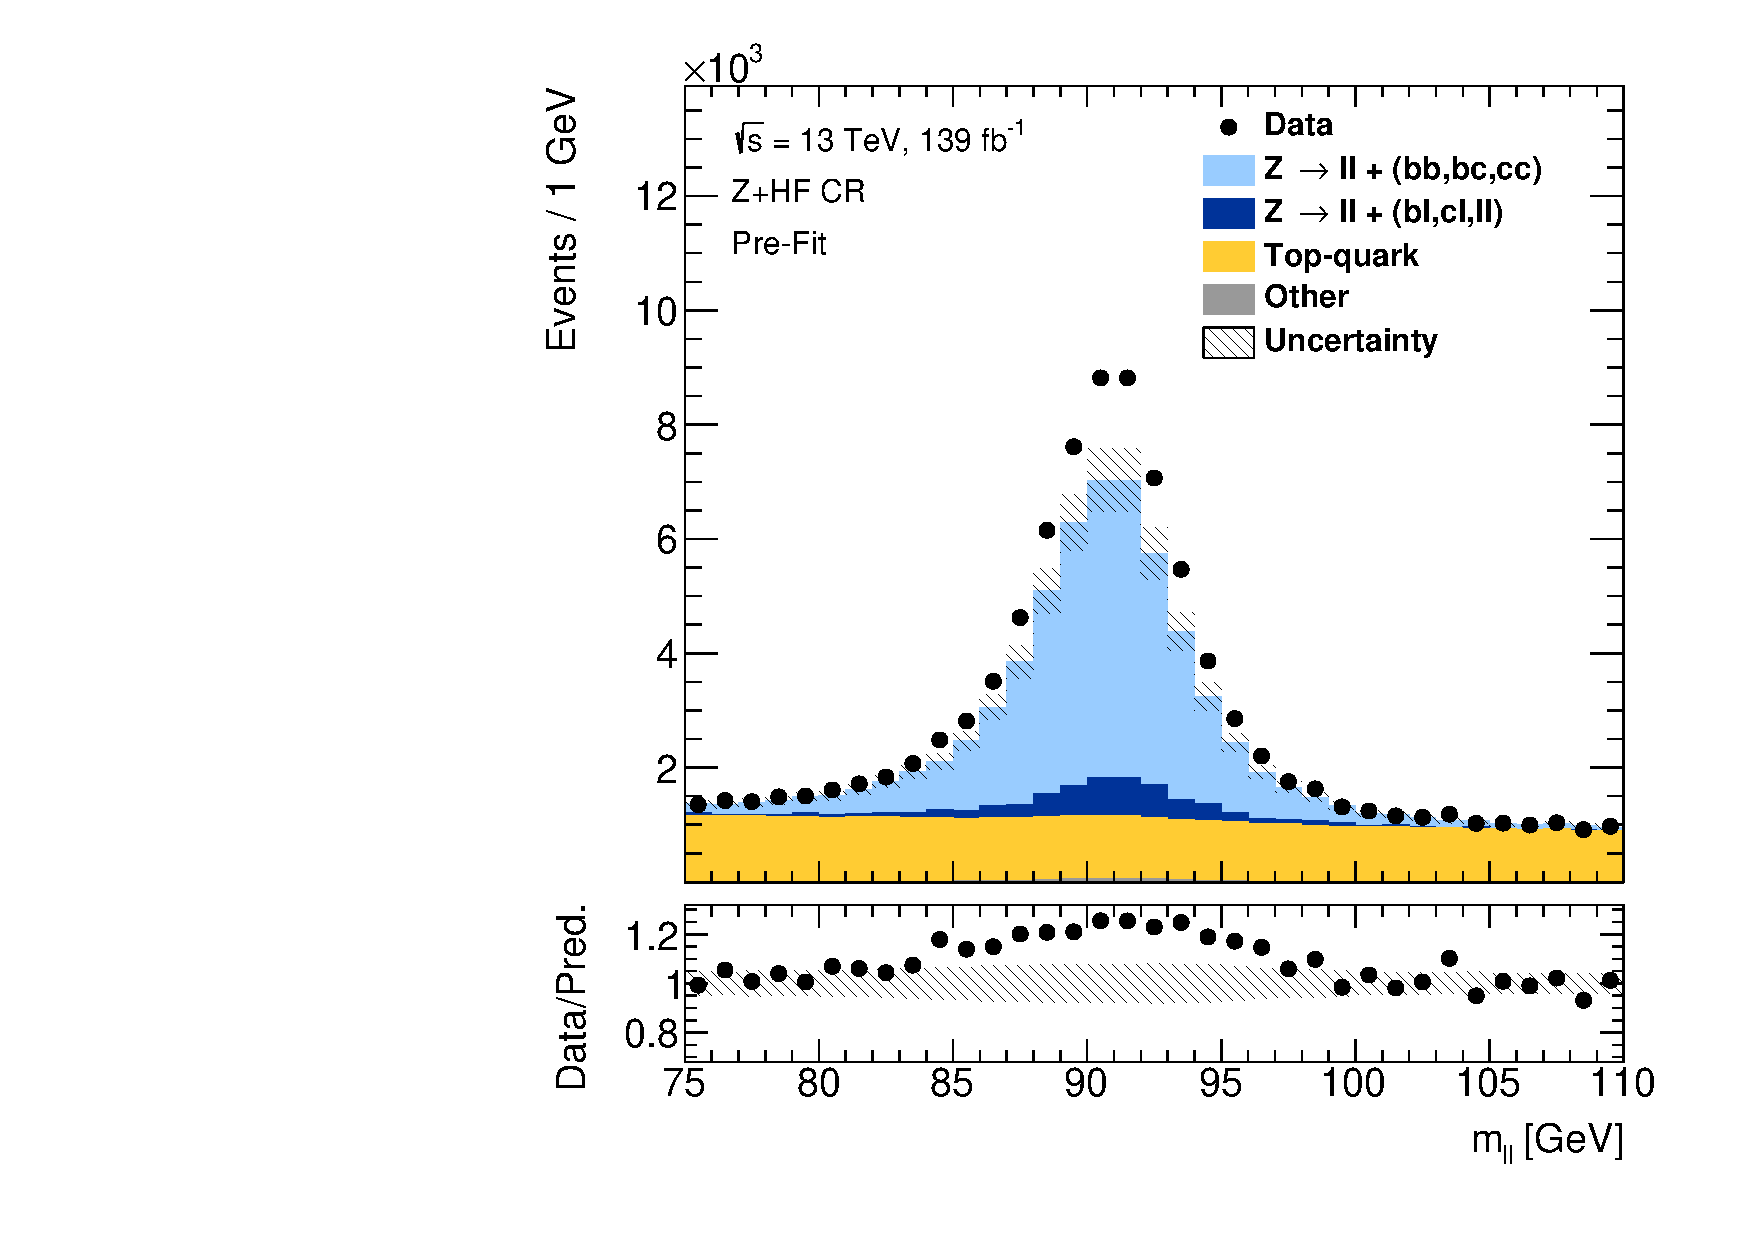
\includegraphics[width=\textwidth]{zhfcr/Region_BMin0_incJet1_Y2015_DZllbbCR_T2_L2_distmLL_J2_Prefit_fixed}
    \subcaption{Pre-fit}
    \label{fig:zcr_mll_prefit}
  \end{subfigure}\hfill%
  \begin{subfigure}{.485\textwidth}
    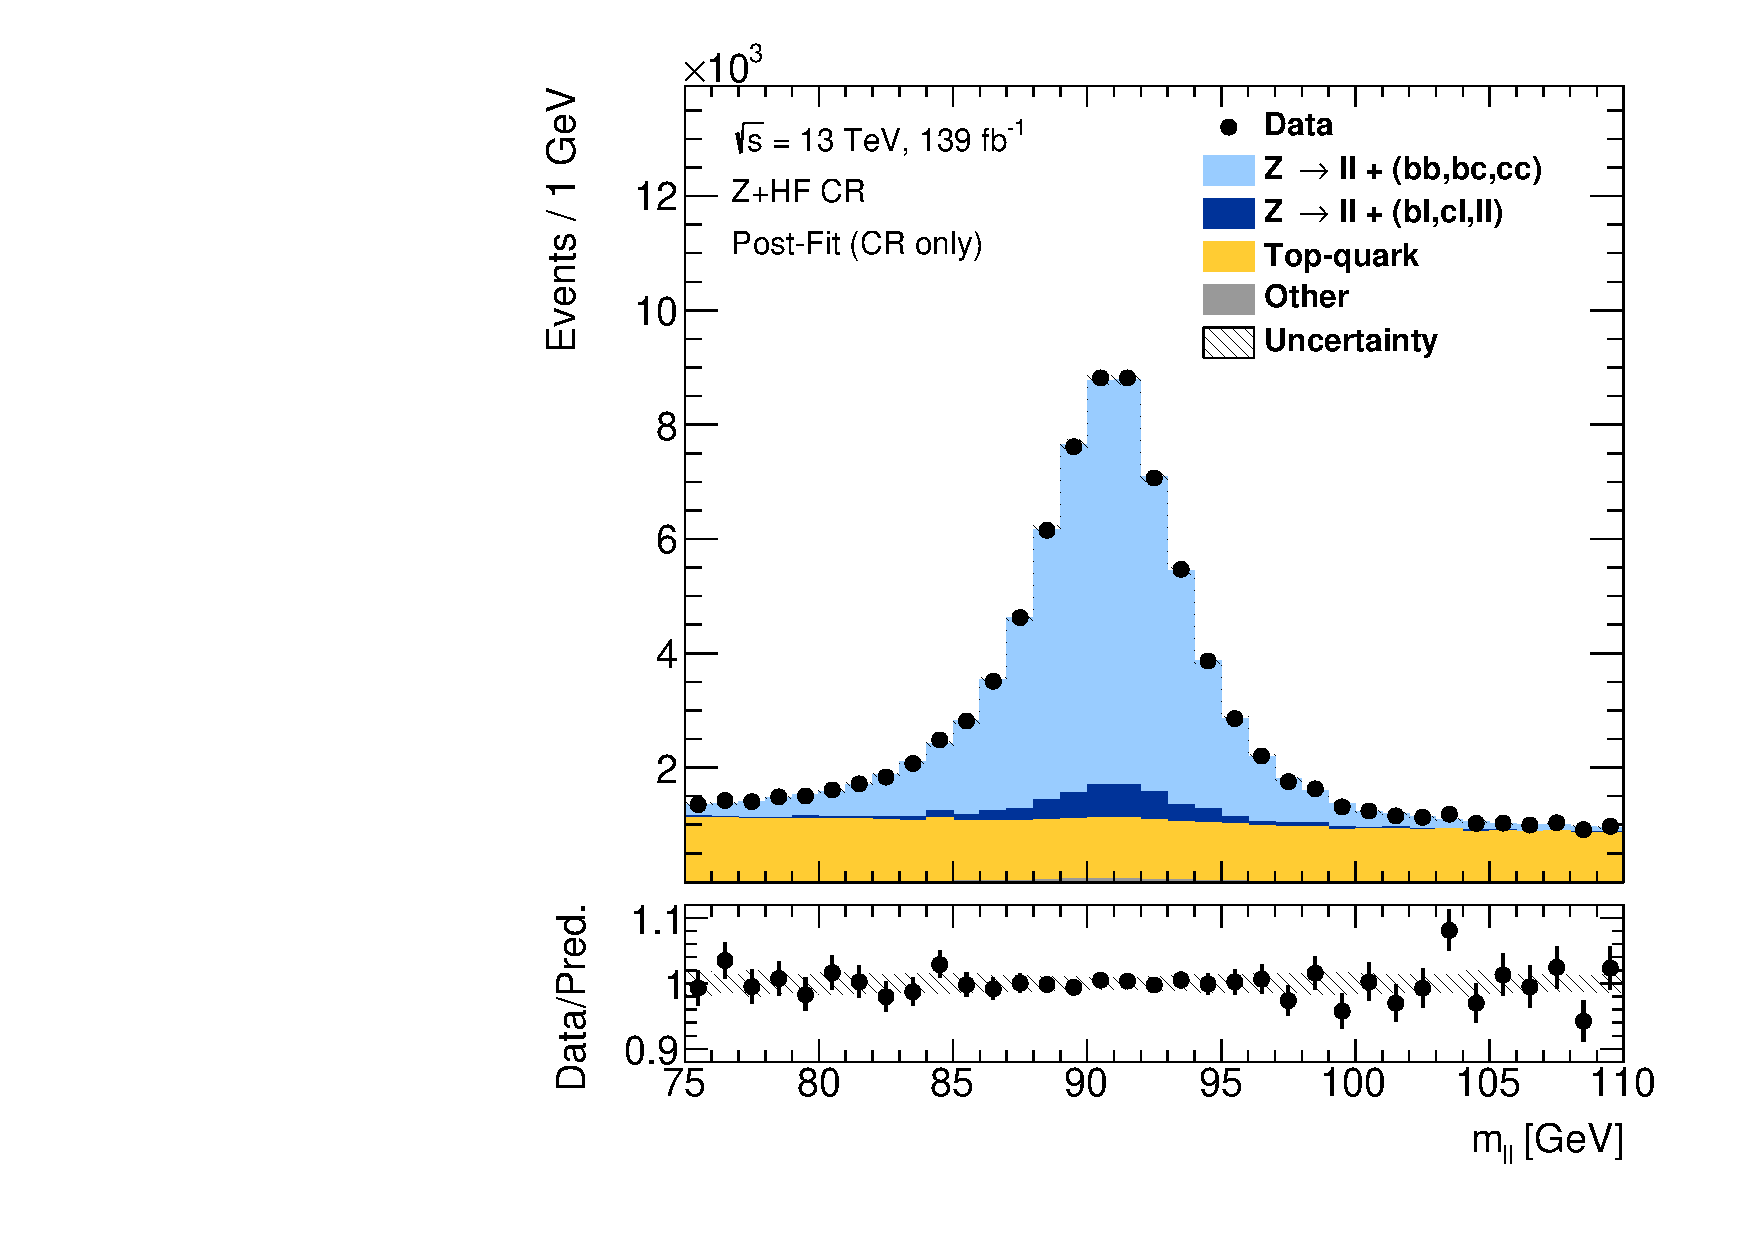
\includegraphics[width=\textwidth]{zhfcr/Region_BMin0_incJet1_Y2015_DZllbbCR_T2_L2_distmLL_J2_GlobalFit_conditionnal_mu0_fixed}
    \subcaption{Post-fit (\ZHF CR only)}
    \label{fig:zcr_mll_postfit}
  \end{subfigure}

  \caption[Distribution of the invariant di-lepton mass in the \ZHF~CR.]{
    Distribution of the invariant di-lepton mass for the combination of
    electron- and muon-channel in the \ZHF CR before (a) and after (b)
    performing a likelihood fit restricted to the CR.  All statistical and
    systematic uncertainties are included.}

  % The contribution of \Zjets is sub-divided into cases where both $b$-jet
  % candidates are matched to heavy flavour quarks ($b$ or $c$) and cases where
  % at most one candidate is matched to heavy flavour quarks at generator-level.
  % Prior to the fit, the \Zjets background is normalised to cross section
  % predictions at NNLO~\cite{Anastasiou:2003ds}.
\end{figure}

% ATLAS_norm_Zhf    1.3856e+00 +/-  1.19e-01
% ATLAS_norm_ttbar    9.7290e-01 +/-  3.92e-02
% Included in the SR fits: Systematic uncertainties are introduced at a later stage...
The \ZHF CR is included in the simultaneous likelihood fit of SRs and CRs to
provide constraints on the normalisation of the \ZHF background. Details on
systematic uncertainties and the fit model are discussed
in~\Cref{sec:uncertainties,sec:statistical_analysis}. Restricting the fit to the
CR yields estimates of the normalisation factors of \num{1.39 \pm 0.12} and
\num{0.97 \pm 0.04} for \ZHF and \ttbar, respectively. The quoted normalisation
factors include all statistical and systematic
uncertainties. \Cref{tab:zcr_yields} and \Cref{fig:zcr_mll_postfit} show the
event yields and \mll distribution after the fit.

% When performing the likelihood fit in the CR only, the
% estimated normalisation factors are~\num{1.39 \pm 0.12} for the \ZHF
% and~\num{0.97 \pm 0.04} for the \ttbar background. The abundance of
% \ttbar events in the CR provides stringent constraints
% on the normalisation of the \ttbar background in addition to
% constraining the normalisation of the \ZHF background. The post-fit
% event yields and \mll distribution is shown in~\Cref{tab:zcr_yields}
% and~\Cref{fig:zcr_mll_postfit}, respectively.

%%% Local Variables:
%%% mode: latex
%%% TeX-master: "../../phd_thesis"
%%% End:
